%%%%%%%%%%%%%%%%%%%%%%%%%%%%%%%%%%%%%%%%%%%%%%%%%%%%%%%%%%%%%%%%%%%%%%%
% Ansys Techcon 2022 - PyVista – Visualizing CAE and Results with Python
%%%%%%%%%%%%%%%%%%%%%%%%%%%%%%%%%%%%%%%%%%%%%%%%%%%%%%%%%%%%%%%%%%%%%%%
\documentclass[t]{beamer}

\usetheme{Ansys2022}

\usepackage{animate}
\usepackage{svg}
\usepackage{bbding,pifont}
\usepackage{minted}
\usepackage{xcolor}
\usepackage{pdfpages}
\usepackage{listings}
\usepackage{hyperref}

\usepackage{tikz}
\usetikzlibrary{intersections}
\usetikzlibrary{shapes.geometric, arrows,positioning}

\usepackage[edges]{forest}
\hypersetup{
    colorlinks=true,
    linkcolor=blue,
    filecolor=magenta,
    urlcolor=cyan,
}


\urlstyle{same}
\setbeamercolor{background canvas}{bg=}

\definecolor{bleudefrance}{rgb}{0.19, 0.55, 0.91}

%%%%%%%%%%%%%%%%%%%%%%%%%%%%%%%%%%%%%%%%%%%%%%%%%%%%%%%%%%%%%%%%%%%%%%%%%%%%%%%

\tikzset{
  startstop/.style={
    rectangle,
    rounded corners,
    minimum width=3cm,
    minimum height=0.75cm,
    align=center,
    draw=black,
    fill=ANSYS@Gold,
    },
  process/.style={
    rectangle,
    minimum width=3cm,
    minimum height=0.75cm,
    align=center,
    draw=black,
    fill=ANSYS@Blue,
    text=white,
    },
  decision/.style={
    diamond,
    aspect=4,
    minimum width=3cm,
    minimum height=1cm,
    align=center,
    draw=black,
    fill=ANSYS@Blue,
    text=white,
    },
  arrow/.style={thick,->,>=stealth},
  dec/.style={
    ellipse,
    align=center,
    draw=black,
    fill=ANSYS@Bronze,
    },
}

\begin{document}

%%%%%%%%%%%%%%%%%%%%%%%%%%%%%%%%%%%%%%%%%%%%%%%%%%%%%%%%%%%%%%%%%%%%%%%%%%%%%%%
%% Title Slide

\title{PyVista – Visualizing CAE and Results with Python}
%% \subtitle{}
\author{Alex Kaszynski}
\date{\today}

\titleframe{}


%%%%%%%%%%%%%%%%%%%%%%%%%%%%%%%%%%%%%%%%%%%%%%%%%%%%%%%%%%%%%%%%%%%%%%%%%%%%%%%
%% Table of contents

\begin{frame}{Table of Contents}
  \tableofcontents
  \vspace{200pt}  %% force top tight
\end{frame}

%%%%%%%%%%%%%%%%%%%%%%%%%%%%%%%%%%%%%%%%%%%%%%%%%%%%%%%%%%%%%%%%%%%%%%%%%%%%%%%
\section{PyVista - Introduction}

%%%%%%%%%%%%%%%%%%%%%%%%%%%%%%%%%%%%%%%%%%%%%%%%%%%%%%%%%%%%%%%%%%%%%%%%%%%%%%%
\begin{frame}
  \frametitle{PyVista - Introduction}

  \begin{columns}[T]

    \begin{column}{.5\textwidth}
      \vspace{-10pt}
      \inputminted[fontsize=\footnotesize]{python}{code/pv_example1.py}
    \end{column}

    \begin{column}{.4\textwidth}
      \vspace{-20pt}
      \centering
      
\includegraphics[height=0.2\textheight]{figures/pyvista_logo.png}
    \end{column}

  \end{columns}
  \vspace{5pt}

  PyVista allows you to rapidly load meshes and handles much of the “grunt
  work” of setting up plots, connecting classes and pipelines, and cleaning up
  plotting windows.

  \vspace{5pt}

  \begin{exampleblock}{PyVista allows you to:}
    \begin{itemize}
    \item Easily load a wide variety of datasets and file types.
    \item Leverage powerful VTK filters and perform complex data operations.
    \item Quickly set up simple or complex plots.
    \end{itemize}
  \end{exampleblock}

\end{frame}


%%%%%%%%%%%%%%%%%%%%%%%%%%%%%%%%%%%%%%%%%%%%%%%%%%%%%%%%%%%%%%%%%%%%%%%%%%%%%%%
\subsection{Quick Example}
\begin{frame}
  \frametitle{Quick Example - Path Operation}

  \begin{columns}[T]
    \begin{column}{.5\textwidth}
      \vspace{-15pt}
      \inputminted[fontsize=\footnotesize]{python}{code/path_op.py}
    \end{column}

    \begin{column}{.5\textwidth}
      \vspace{-15pt}
      \centering
      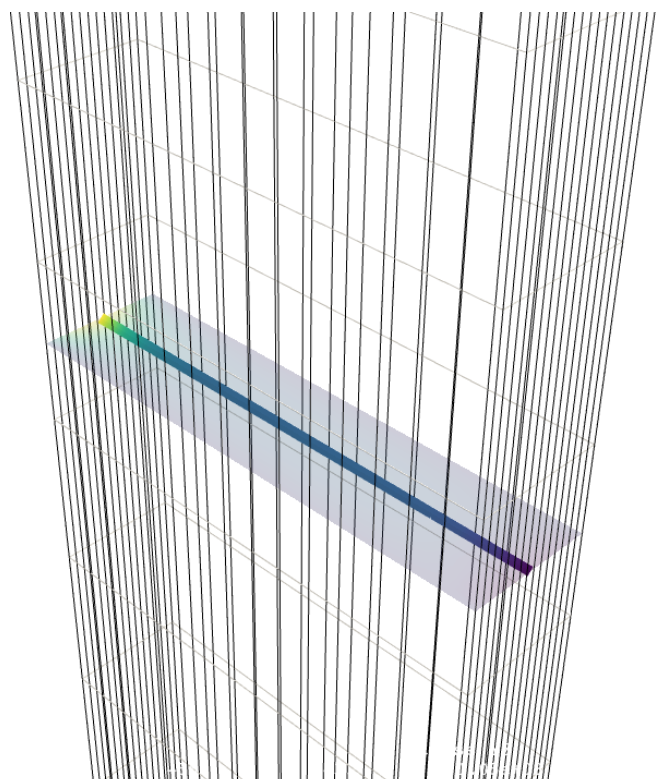
\includegraphics[width=0.75\textwidth]{figures/path_op.png}
    \end{column}
  \end{columns}

\end{frame}

%%%%%%%%%%%%%%%%%%%%%%%%%%%%%%%%%%%%%%%%%%%%%%%%%%%%%%%%%%%%%%%%%%%%%%%%%%%%%%%
\begin{frame}
  \frametitle{Quick Example - Path Operation vs PyMAPDL}

  \begin{columns}[T]
    \begin{column}{.5\textwidth}
      \vspace{-15pt}
      \inputminted[fontsize=\footnotesize]{python}{code/path_op_vs_pymapdl.py}
    \end{column}

    \begin{column}{.5\textwidth}
      \vspace{-15pt}
      \centering
      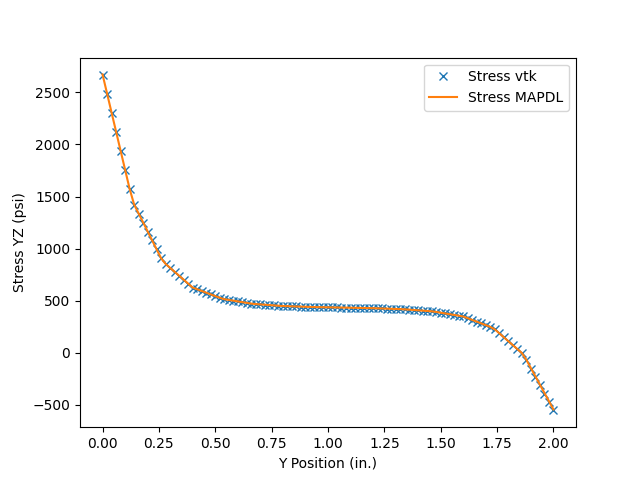
\includegraphics[width=1.0\textwidth]{figures/path_op_vs_pymapdl.png}
    \end{column}
  \end{columns}


\end{frame}


%%%%%%%%%%%%%%%%%%%%%%%%%%%%%%%%%%%%%%%%%%%%%%%%%%%%%%%%%%%%%%%%%%%%%%%%%%%%%%%
\subsection{Comparison - VTK vs. PyVista}
\begin{frame}
  \frametitle{Comparison - VTK vs. PyVista}
  \begin{columns}[T]
    \begin{column}{.5\textwidth}
      \vspace{-15pt}
      \inputminted[fontsize=\footnotesize]{python}{code/vtk_example.py}
    \end{column}

    \begin{column}{.5\textwidth}
      \vspace{-15pt}
      \inputminted[fontsize=\footnotesize]{python}{code/pv_example.py}
      \vspace{-5pt}
      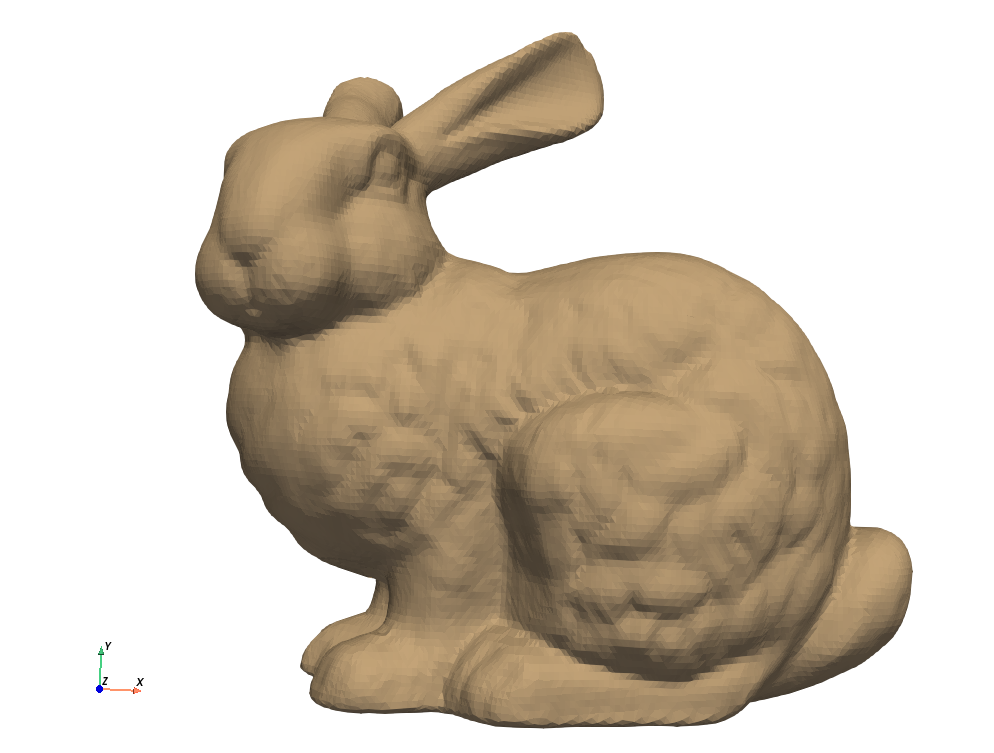
\includegraphics[width=\textwidth]{figures/pv_example.png}
    \end{column}
  \end{columns}

\end{frame}

%%%%%%%%%%%%%%%%%%%%%%%%%%%%%%%%%%%%%%%%%%%%%%%%%%%%%%%%%%%%%%%%%%%%%%%%%%%%%%%
\subsection{Where is it already used?}
\begin{frame}
  \frametitle{PyVista - Current Usage}

  \vspace{-8pt}
  PyVista is already being used by:
  \vspace{-8pt}

  \begin{columns}[T]
    \begin{column}{.3\textwidth}
        \begin{exampleblock}{ACE \& Partners}
        \inputminted[fontsize=\tiny]{python}{code/dpf_simple.py}
        \centering
        \href{https://www.padtinc.com/2022/07/18/ansys-scripting-python-p1-solve-post/}{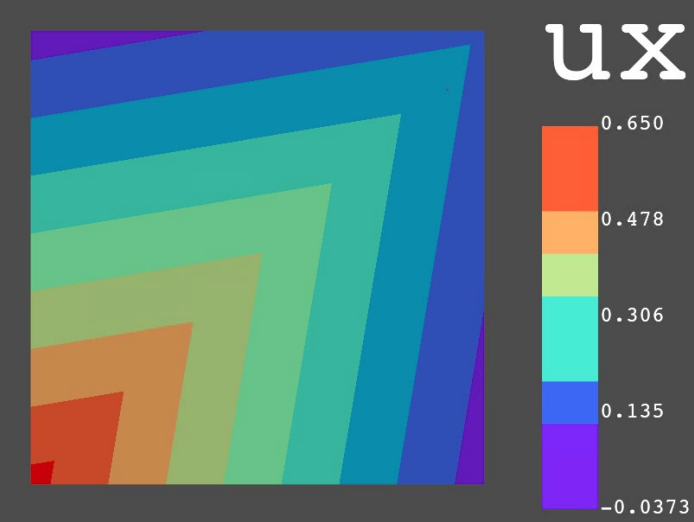
\includegraphics[width=0.95\textwidth]{figures/dpf_simple.png}}
        \end{exampleblock}
      \end{column}

    \begin{column}{.3\textwidth}
        \begin{exampleblock}{PyAnsys}
        \inputminted[fontsize=\tiny]{python}{code/pymapdl_eo_disc.py}
        \centering
        \href{https://github.com/pyansys/ray-segments-pyvista}{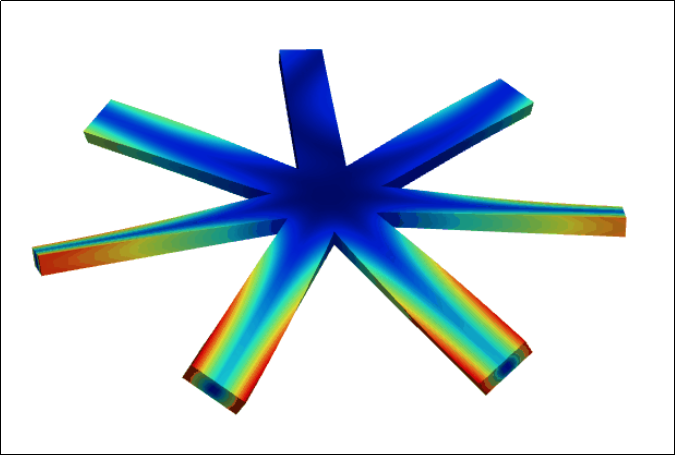
\includegraphics[width=0.95\textwidth]{figures/pymapdl_eo_disc.png}}
        \end{exampleblock}
      \end{column}

    \begin{column}{.3\textwidth}
        \begin{exampleblock}{OnScale}
        \inputminted[fontsize=\tiny]{python}{code/onscale_pyvista.py}
        \centering
        \href{https://github.com/pyansys/ray-segments-pyvista}{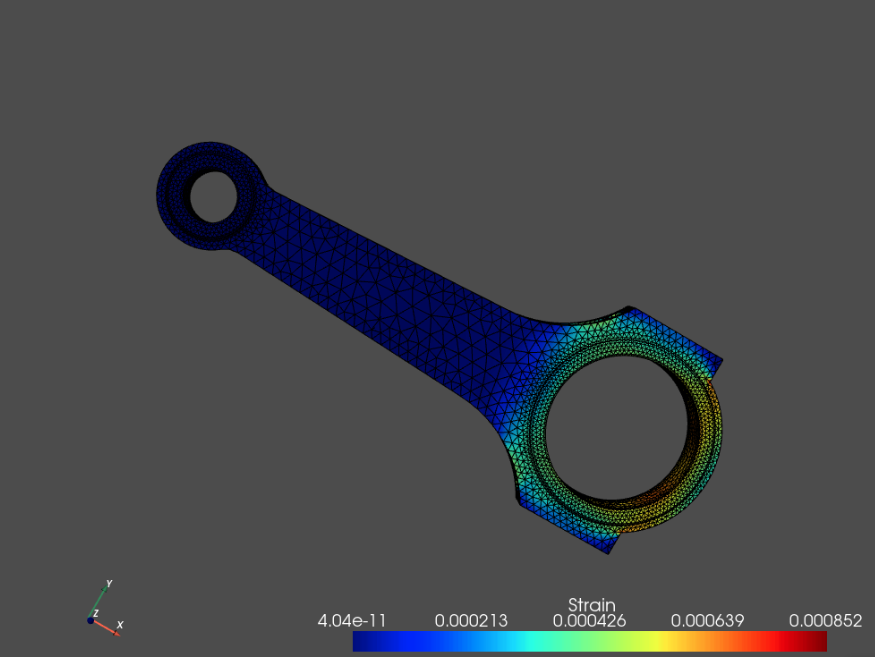
\includegraphics[width=0.95\textwidth]{figures/onscale_pyvista.png}}
        \end{exampleblock}
      \end{column}

  \end{columns}

\end{frame}

%%%%%%%%%%%%%%%%%%%%%%%%%%%%%%%%%%%%%%%%%%%%%%%%%%%%%%%%%%%%%%%%%%%%%%%%%%%%%%%
\section{Getting Started}

\begin{frame}
  \frametitle{APIs - Definition and Examples}
  \tableofcontents[currentsection]
  \vspace{200pt}  %% force top tight
\end{frame}

%%%%%%%%%%%%%%%%%%%%%%%%%%%%%%%%%%%%%%%%%%%%%%%%%%%%%%%%%%%%%%%%%%%%%%%%%%%%%%%
\begin{frame}[fragile=singleslide]
  \frametitle{Installation}
  \vspace{-10pt}

  \begin{columns}[T]
    \begin{column}{.5\textwidth}
      \vspace{-10pt}
      \begin{exampleblock}{pip}
        \begin{lstlisting}[basicstyle=\ttfamily\footnotesize]
pip install pyvista
        \end{lstlisting}
      \end{exampleblock}

    \end{column}

    \begin{column}{.5\textwidth}
      \vspace{-10pt}
      \begin{exampleblock}{conda}
        \begin{lstlisting}[basicstyle=\ttfamily\footnotesize]
conda install -c conda-forge pyvista
        \end{lstlisting}
      \end{exampleblock}

    \end{column}
  \end{columns}

  \vspace{5pt}

  \centering
  \href{https://asciinema.org/a/507562}{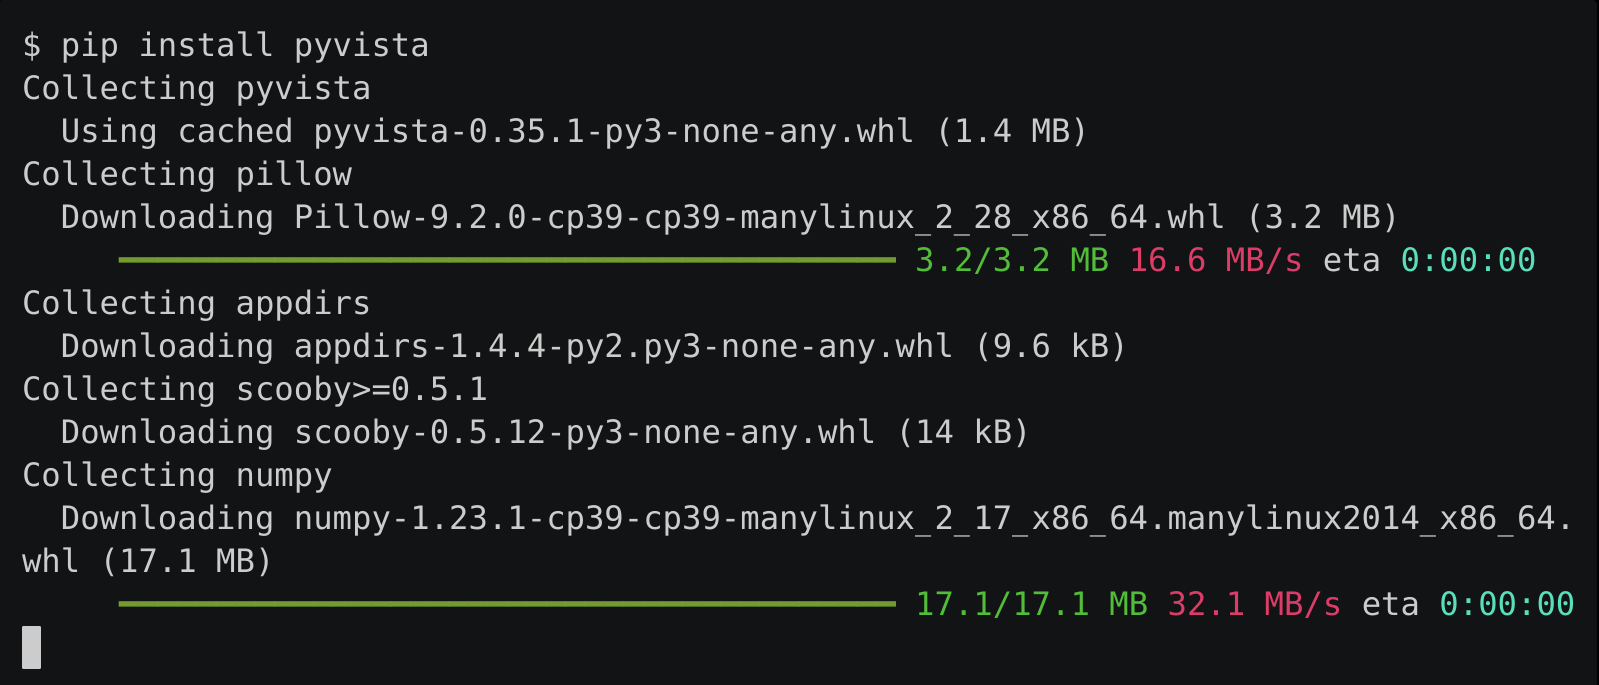
\includegraphics[width=0.76\textwidth]{figures/install_pyvista.png}}

\end{frame}

%%%%%%%%%%%%%%%%%%%%%%%%%%%%%%%%%%%%%%%%%%%%%%%%%%%%%%%%%%%%%%%%%%%%%%%%%%%%%%%
\lastframe{}

\end{document}
